\documentclass[thesis.tex]{subfiles}

\begin{document}

\chapter{Evaluation}\label{chap:eva}

In this chapter, the performance of the developed application is analysed using various metrics. Section~\ref{sec:testsystem} defines the serial and GPU test systems. Section \ref{sec:fp32issues} illustrates the main problems with performing SE on CUDA using FP32 operations. Section~\ref{sec:perfMetr} lists the metrics against which the performances are assessed. Section \ref{sec:centPerf} examines the application’s performances on grids of various sizes using centralized SE. Section \ref{sec:decPerf} presents the performance improvements using decentralized SE.

\section{Test System} \label{sec:testsystem}
As described earlier in Section~\ref{sec:hardware}, the target GPUs are GTX 1070 (1920 cores) and Tesla V100 (5120 cores) of compute-capabilities 6.1 and 7.0 respectively. GTX 1070 is a commonplace GPU mostly used for gaming whereas V100 is NVIDIA’s flagship product HPC applications. In comparison to the specifications of these GPUs, the serial algorithm is executed on a host with the specifications as follows:
\begin{itemize}
	\item CPU: Intel Xeon E5-2620: 2.40 GHz, 24 CPUs
	\item RAM: 32 GB
\end{itemize}
The inputs to GPU-based TM-WLS state estimator are pseudo-measurements obtained after noise is added to power-flow results in the serial MATLAB algorithm. To evaluate the accuracy the state estimator output, the final results are compared with that of the serial algorithm.

\section{Issues with FP32 CUDA-accelerated SE}\label{sec:fp32issues}
The application provides two variants of computations, i.e. FP32 and FP64. While FP64 computations are found to match the serial algorithm’s results, FP32 computations suffer from the following problems:
\begin{itemize}
	\item Lack of convergence with $\epsilon = 0.001$
	\item Relatively larger errors in comparison to the reference results from serial algorithm.
\end{itemize}
In particular, FP32 computations do not converge with $\epsilon = 0.001$ as the maximum residual error $max(|\Delta \textbf{\textit{x}}|)$ obtained per WLS iteration in the later stages is found to take random values between 0.5 and 0.01. This problem arises in FP32 computations due to the following reasons:
\begin{enumerate}
	\item Relatively smaller size of bits available for data storage in FP32 results in larger representation errors due to rounding operations.
	\item The results depends on the sequence of basic arithmetic operations as the rounding errors get propagated differently with different orders of operations. This is especially unpredictable since the scheduling of warps that perform the computations depend on the available GPU resources.
\end{enumerate}
\begin{figure}[H]
	\centering
	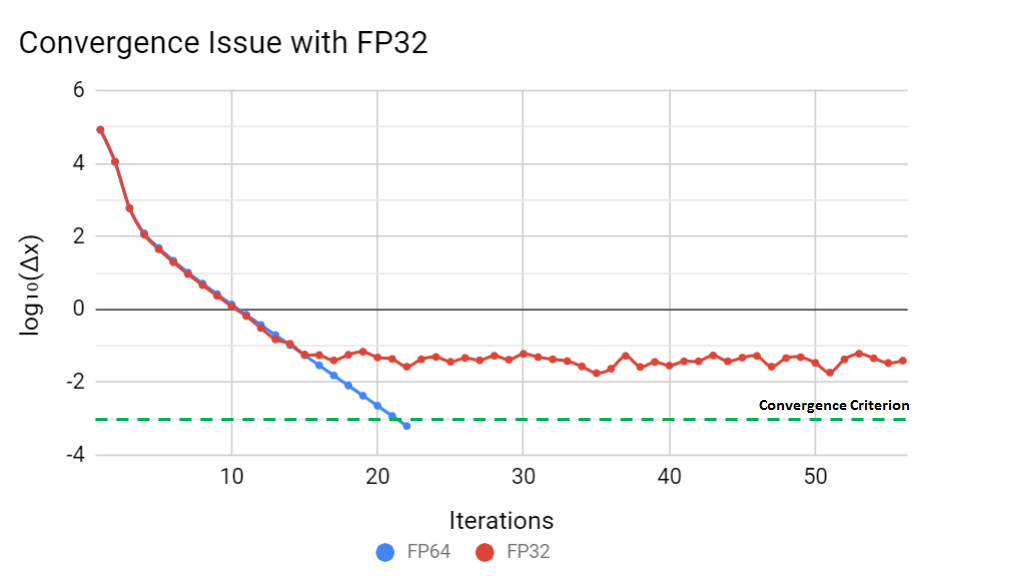
\includegraphics[scale=0.55]{convissue}
	\caption{Lack of convergence with FP32}
	\label{fig:convissue}
\end{figure}
Hence, although relatively larger errors in state vector due to intermediate rounding errors cannot be resolved, the issue with lack of convergence with FP32 computations may be solved by increasing the predetermined constant $\epsilon$ from 0.001 to 0.5. Such significant increment may further introduce an impact on the accuracy of the final results which is evaluated in the subsequent section~\ref{subsec:volPhaErrors}.


\section{Performance Metrics}\label{sec:perfMetr}
In order to examine the impact of massive parallelization using GPUs and its two different precisions, it is necessary to define certain metrics against which the performance and accuracy of the application in centralized as well as decentralized modes can be analyzed. They are described as follows:
\subsection{Speed-up}
This is an important metric to decide if usage of parallelization is beneficial. It is defined as the ratio of the time taken by serial algorithm to the time taken by the implemented CUDA application. Two speed-ups for both precisions respectively can be obtained as follows:
\begin{equation*}
S_{64} = \frac{t_{Serial}}{t_{CUDA_{64}}}
\end{equation*}
\begin{equation*}
S_{32} = \frac{t_{Serial}}{t_{CUDA_{32}}}
\end{equation*}

where $S$ suffixed with the precisions are speed-ups and $t_{CUDA_{32}}$ and $t_{CUDA_{64}}$ are the times taken using FP32 and FP64 computations respectively inclusive of forward and backward data transfers over PCIe bus. Similarly, $t_{Serial}$ is the time taken by the serial algorithm.

\subsection{Maximum and Minimum Errors}\label{subsec:speedups}
The serial algorithm computes the state vector in double precision and it serves as the reference. The results obtained using 2 CUDA-supported precisions must be compared with the reference result to assess the accuracy of the results. The extent of the errors introduced can be presented using an interval of maximum and minimum errors.

\subsection{Space Complexity}
In order to process datasets from grids of various sizes, different amounts of VRAM is required. With increase in matrix dimensions and the associated dense algebraic computations, the memory consumption is expected to increase with the grid-sizes. The nature of relationship between the grid-sizes and the memory-space requirements should be investigated.


\section{Performance Analysis of Centralized SE}\label{sec:centPerf}
In order to characterize the performance of SE on CUDA, its performance must be compared to that of the serial algorithm. Since the matrices involved in SE are highly sparse in nature, the serial algorithm is allowed to use sparse matrices (CSC 0-based format) in order to reduce computational burden. However, the CUDA implementation in this case uses dense matrices to perform the same computations. 

\subsection{Efficiency Evaluation}\label{subsec:effeval}
The efficiency of computation can be expressed in speed-ups discussed in Section~\ref{subsec:speedups}. The required execution times for various grid-sizes for the serial SE algorithm can be obtained from Matlab. Subsequently, to evaluate the efficiency of the implementation, the following tests are performed:
\begin{enumerate}
	\item SE is perfomed using FP64 computations. In this case, the number of WLS iterations ($n$) is found to be exactly equal to that of the serial algorithm. 
	\item In order to perform SE using FP32 computations, the convergence criterion $\epsilon = 0.001$ cannot be used. As discussed in Section \ref{sec:fp32issues}, increasing the value of $\epsilon$ is a solution but that would lead to unequal number of WLS iterations, thereby making the execution times incomparable. Hence, to maintain comparability, SE is performed using FP32 computations for $n$ iterations by fixing the loop condition.
\end{enumerate}

For both the approaches, the required computation times are recorded as well as the state vectors are saved as CSV files. The speed-ups obtained on CUDA are illustrated in Figure \ref{fig:centralizedSEspeedups} as follows:
\begin{figure}[H]
	\centering
	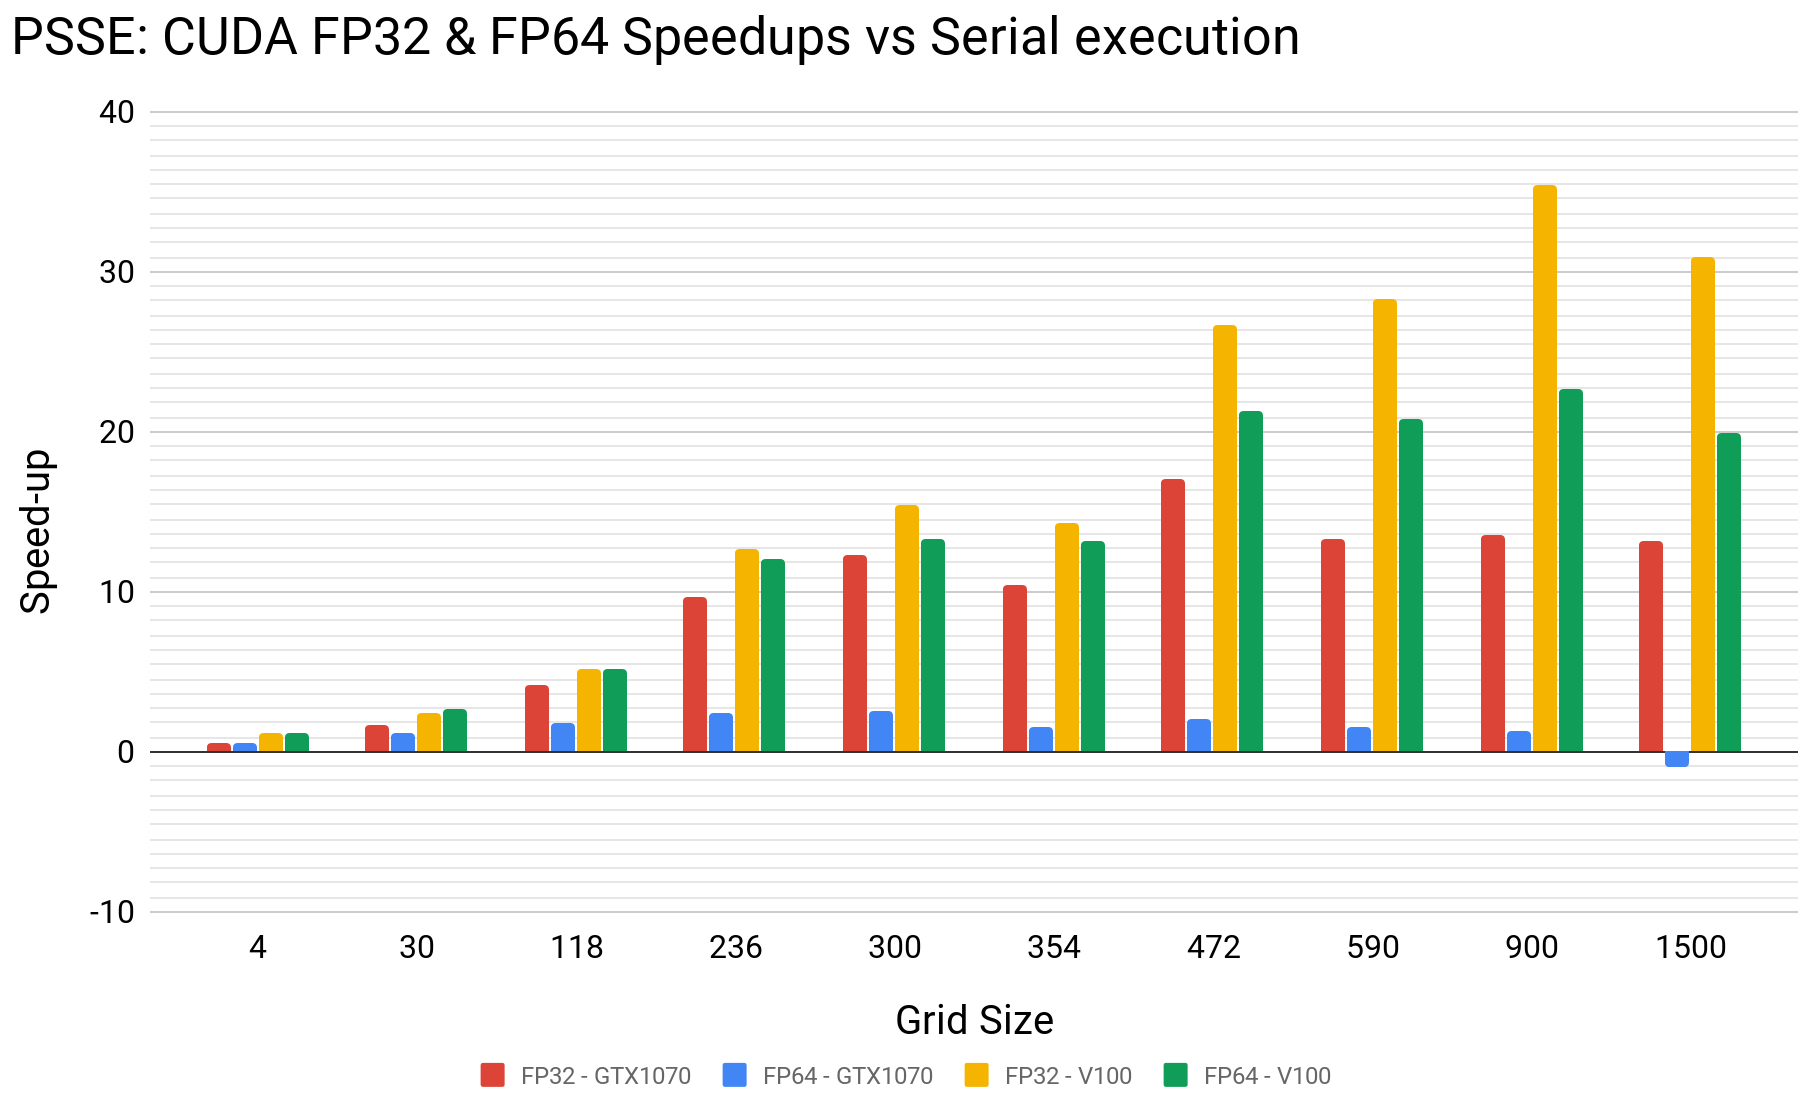
\includegraphics[scale=0.42]{centralizedSEspeedups}
	\caption{Speedups using GTX1070 and V100 vs serial Matlab algorithm}
	\subcaption*{A speedup value between 0 and 1 means slowdown whereas -1 indicates program crash due to VRAM shortage. Values greater than 1 are desired.}
	\label{fig:centralizedSEspeedups}
\end{figure}

Some of the grids used are standard IEEE grids (4, 30, 118, 300) whereas others are constructed through connected replications discussed in Section \ref{subsec:innately}.\\
As observed in Figure \ref{fig:centralizedSEspeedups}, unlike in FP32, execution on GTX1070 crashes while processing 1500-bus grid in FP64. The reason for this execution failure is the required VRAM for FP64 SE computations. GTX1070 has a total of 8GB of VRAM whereas the current state of the implementation demands 9.6GB for processing 1500-bus grid.

In order to understand the times taken by individual arithmetic or non-arithmetic operations, the CUDA kernel launches can be profiled using CLI tool \inlinecode{C}{nvprof} or the user-friendly GUI counterpart - NVIDIA Visual Profiler. However, some operations require launching multiple kernels. In order to examine the total time taken for such operation, CUDA events can be used instead. It is then observed that the majority of the GPU time consumed is by matrix-matrix dot products and linear system solution operations. Especially for FP64 operations, dot products are found to be the most expensive operations as shown in Figure \ref{fig:timconop}.
\begin{figure}[H]
	\centering
	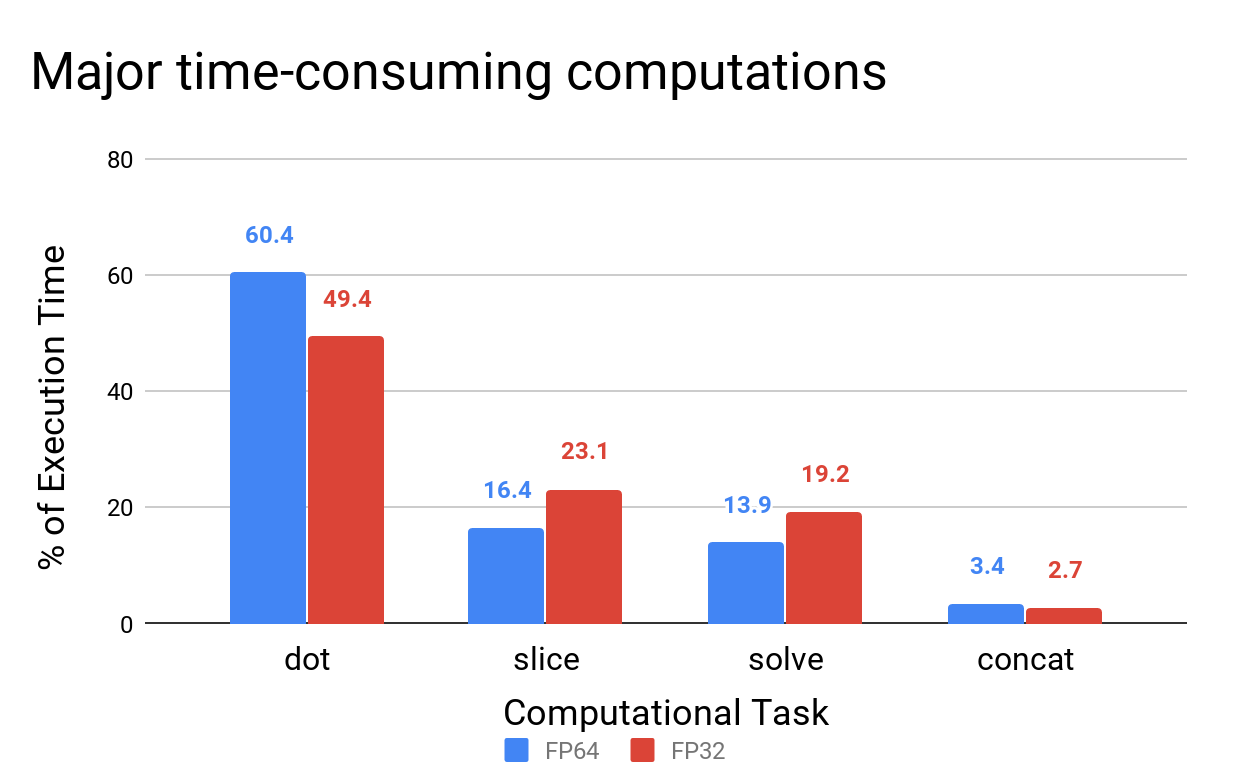
\includegraphics[scale=0.4]{timconop}
	\caption{Most time-consuming operation in FP32 and FP64 operations for 1500-bus grid’s SE on V100 GPU.}
	\label{fig:timconop}
\end{figure}


\subsection{Voltage and Phase Errors}\label{subsec:volPhaErrors}
In Section \ref{subsec:effeval}, equal numbers of WLS iterations are used to obtain comparable execution times. In this section, the value of $\epsilon$ is increased from 0.001 to 0.5 for FP32 operations to examine its impact on accuracy of the results.
The magnitude of errors for FP64 operations is extremely low. FP32 operations on the other hand introduces about 2 orders larger errors. The following figures~\ref{fig:centralizedvoltageerrors} and \ref{fig:centralizedphaseerrors} illustrate the errors in the state vector for a 236-bus grid SE using both the precisions and convergence criterions $\epsilon_{32} = 0.5$ and $\epsilon_{64} = 0.001$ respectively:


\begin{figure}[H]
	\centering
	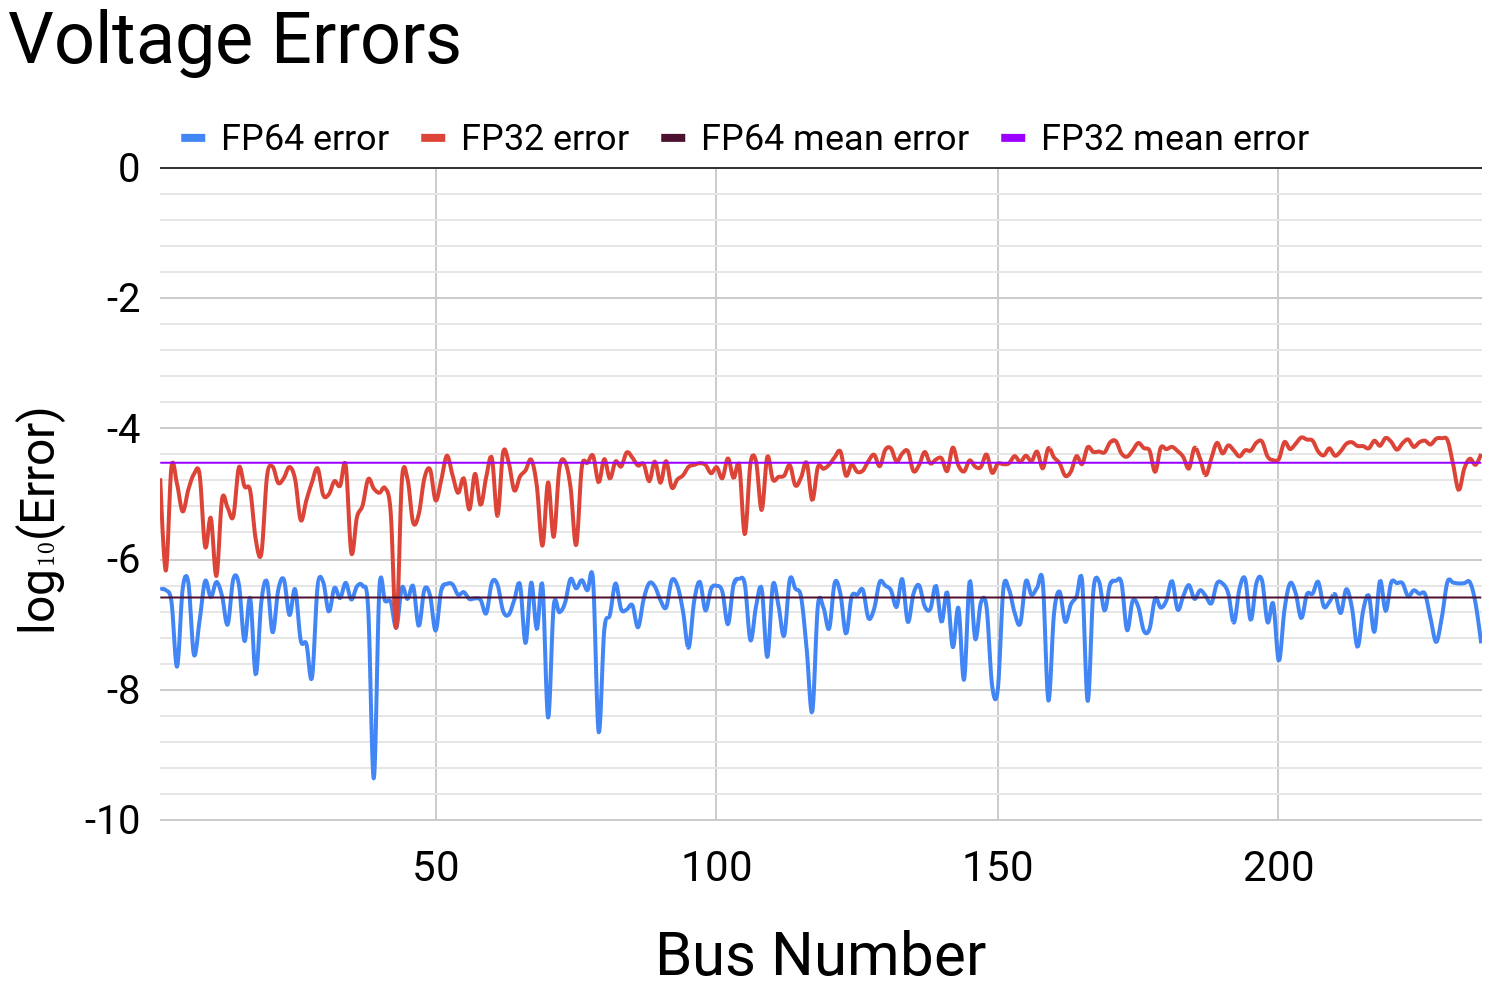
\includegraphics[scale=0.35]{centralizedvoltageerrors}
	\caption{Voltage errors using FP32 \& FP64 operations in 236-bus grid}
	\label{fig:centralizedvoltageerrors}
\end{figure}

\begin{figure}[H]
	\centering
	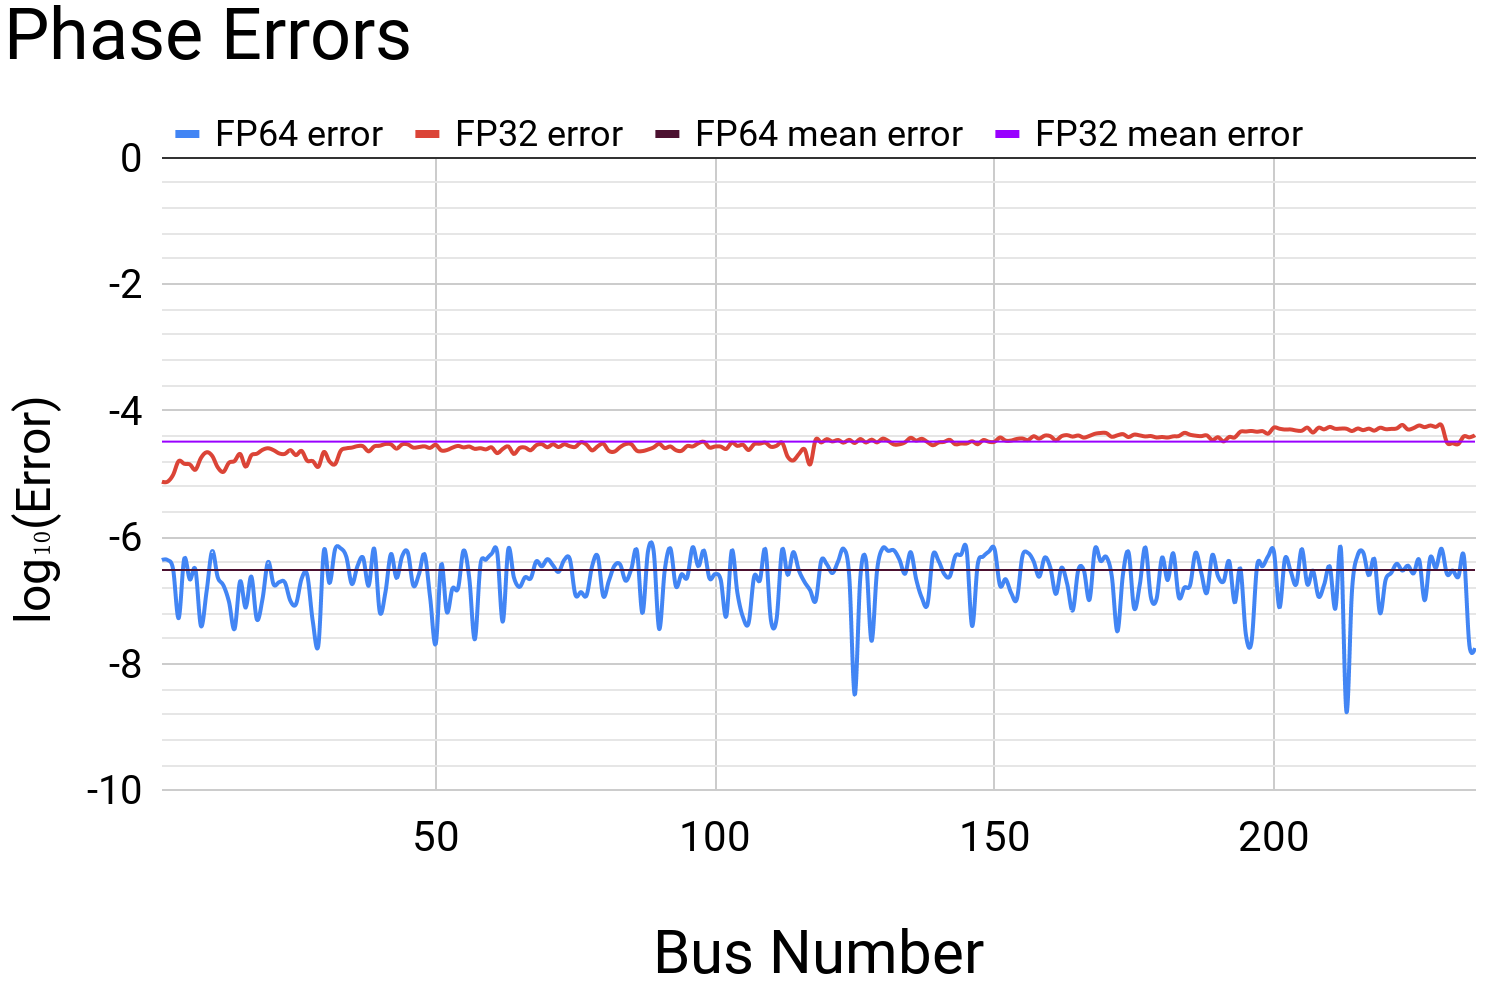
\includegraphics[scale=0.35]{centralizedphaseerrors}
	\caption{Phase errors using FP32 \& FP64 operations in 236-bus grid}
	\label{fig:centralizedphaseerrors}
\end{figure}

The maximum and minimum relative errors (in \%) for the voltage and phase values observed in the above figures are presented below in Table~\ref{relativeerrors}:
{\renewcommand{\arraystretch}{1.3}%
\begin{table}[H]
	\centering
	\begin{tabular}{|l|r|r|}
		\hline 
		& FP32 Computations & FP64 Computations \\ 
		\hline 
		Range of Voltage Error(\%) & [ 4.78E-08, 4.83E-05] & [2.34E-10, 3.09E-07] \\ 
		\hline 
		Range of Phase Error(\%) & [0, 4.14E-03] & [0, 1.12E-04] \\ 
		\hline 
	\end{tabular} 
	\caption{Maximum and minimum voltage \& phase relative errors using FP32 and FP64 operations.}
	\label{relativeerrors}
\end{table}}

Since none of these errors are greater than 1\%, operations from both precision are concluded to produce operationally acceptable values. This is of special importance because apart from being highly precise, FP32 operations are also faster on GPU than FP64 operations for GTX1070 as well as V100. 

\subsection{Reduction in Memory Requirements}
The responsibility of memory management in CUDA is on the programmer. As conceptualised in Section~\ref{dmmse}, the implementation and integration of a custom device memory manager (DMM) that is capable of recycling and reusing memory allocations into the GPU-accelerated SE application can result in significant reduction in memory requirements during computations. This also alleviates the need to launch expensive \inlinecode{C}{cudaFree} and \inlinecode{C}{cudaMalloc} functions after $1^{st}$ WLS iteration. As an example, if the SE algorithm takes 15 iterations to converge, the memory consumptions with and without the DMM for 118 and 236 bus grids are illustrated in Figure \ref{fig:devmemreduc} as follows:

\begin{figure}[H]
	\centering
	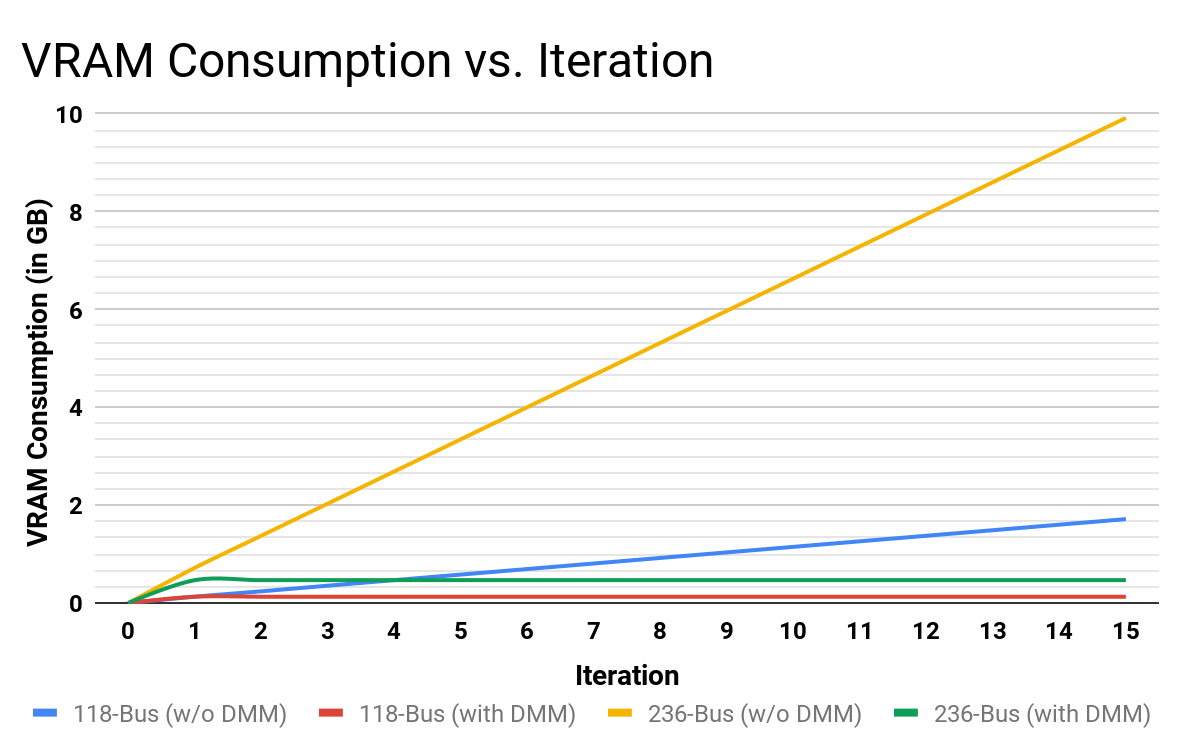
\includegraphics[scale=0.45]{devmemreduc}
	\caption{VRAM consumption with and without DMM for 118 and 236 bus grids.}
	\label{fig:devmemreduc}
\end{figure}


\subsection{Selection of Building-Block Grid }
From Figure \ref{fig:centralizedSEspeedups}, it can be observed that grid-sizes 4 and 30 do not offer notable speedups on GPU. Significant accelerations are observed for 118-bus grid and larger grids. As discussed in Section~\ref{subsec:innately}, large-scale power systems that may be readily partitioned can be constructed using building-block grid sizes that benefit from GPU-accelerated SE. 
Therefore, for evaluation purposes, 118 is chosen as the building-block to generate large-scale power systems. Through connected replication, grids of much higher complexities can be constructed.

\section{Performance Analysis of Decentralized SE}\label{sec:decPerf}
Following the satisfactory analysis of the performance of the CUDA-accelerated centralized SE implementation on various grid-sizes, the next step would be to analyse the change in efficiency using decentralized SE. The approach used to construct large-scale grids through connected replication can be summarized as follows:
\begin{enumerate}
	\item Each building-block grid is connected to another through 2 to 3 edges (or transmission lines). The last edge always connects the $n^{th}$ bus of an $n$-size grid to the first bus of the subsequent grid. The remaining edges connect busses that are arbitrarily chosen. This is done to emulate actual grid structure to some extent.
	\item Alongside active and reactive power measurements from all the terminals and busses, a PMU measuring terminal current and voltage is placed on all the terminals. 
\end{enumerate}

Upon sectorization of the large power grid, certain issues related to SE computations are frequently observed. They are listed as follows:
\begin{enumerate}
	\item Upon decentralization, the order of the matrices such as measurement Jacobian $\textbf{\textit{H}}(\textbf{\textit{x}})$ is reduced. In principle, this should result in reduced computational burden and shorter convergence times. However, it is likely that one or more partitions take significantly longer than the whole to converge. This can lead to undesirable performance. 
	\item In addition to the longer convergence times, it is also likely that one or more of the partitions do not converge. This prevents the merger of the local states to obtain global states due to missing output(s).
	\item If all the local SE computations converge, it is frequently observed that the difference or merge-error between the obtained global state vector after merger and the state vector from centralized SE is large. 
\end{enumerate}


With these issues associated with decentralized SE in mind, the additional considerations made for this part of evaluation are as follows:
\begin{enumerate}
	\item The merge-errors observed in global state vector of decentralized SE in comparison to centralized SE depends on different power-flow situations. For certain situations, the merge-error is very low, i.e. 2-3\% for voltages and $\pm2$ degrees for phases. For the benchmarking purposes, only measurements with such favorable power-flow situations are considered. This renders the analysis of accuracy unnecessary.
	\item As illustrated in the Figure \ref{fig:fp32inconsistency} and \ref{fig:fp64consistency}, unlike FP64 computations, performing decentralized SE using FP32 computations results in varying number of WLS iterations for every partition per program launch. This is observed due to rounding errors arising from undefined order of scheduling of thread-blocks on SMs. Such inconsistency makes the observations and thus the comparisons non-reproducible for FP32 computations. As a result, only FP64 computations are used for analysing speedups through decentralized SE.
\end{enumerate}

\begin{figure}[H]
	\begin{subfigure}{.5\textwidth}
		\centering
		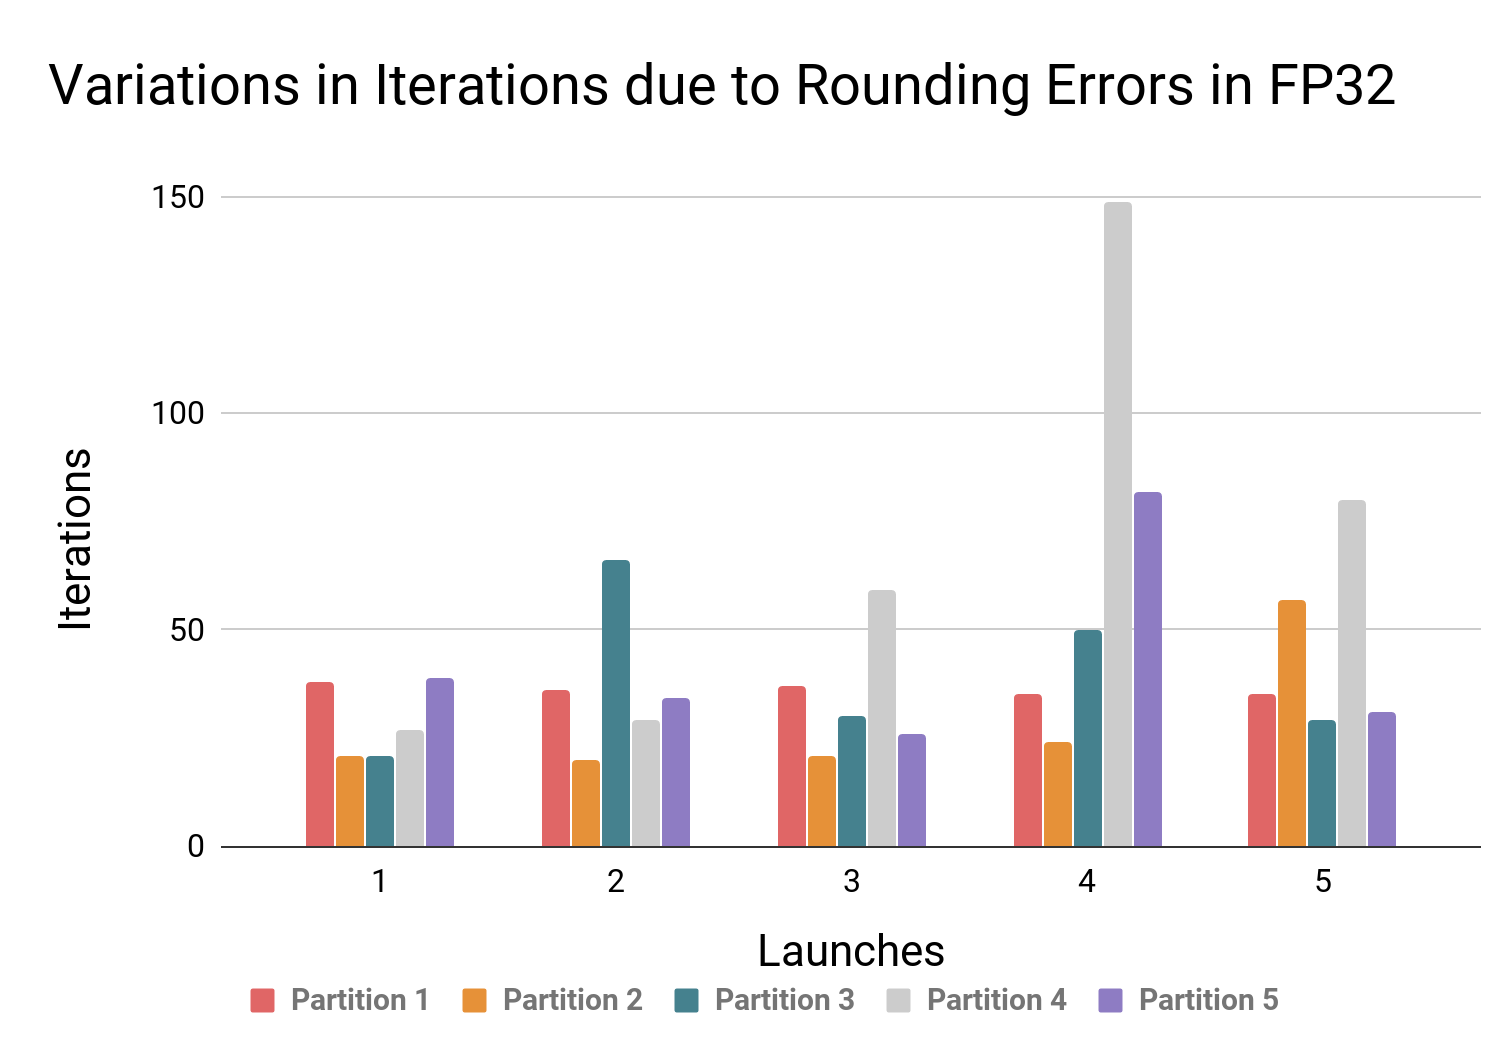
\includegraphics[width=.9\linewidth]{fp32inconsistency}
		\caption{Inconsistency in WLS iterations}
		\label{fig:fp32inconsistency}
	\end{subfigure}
	\begin{subfigure}{.5\textwidth}
		\centering
		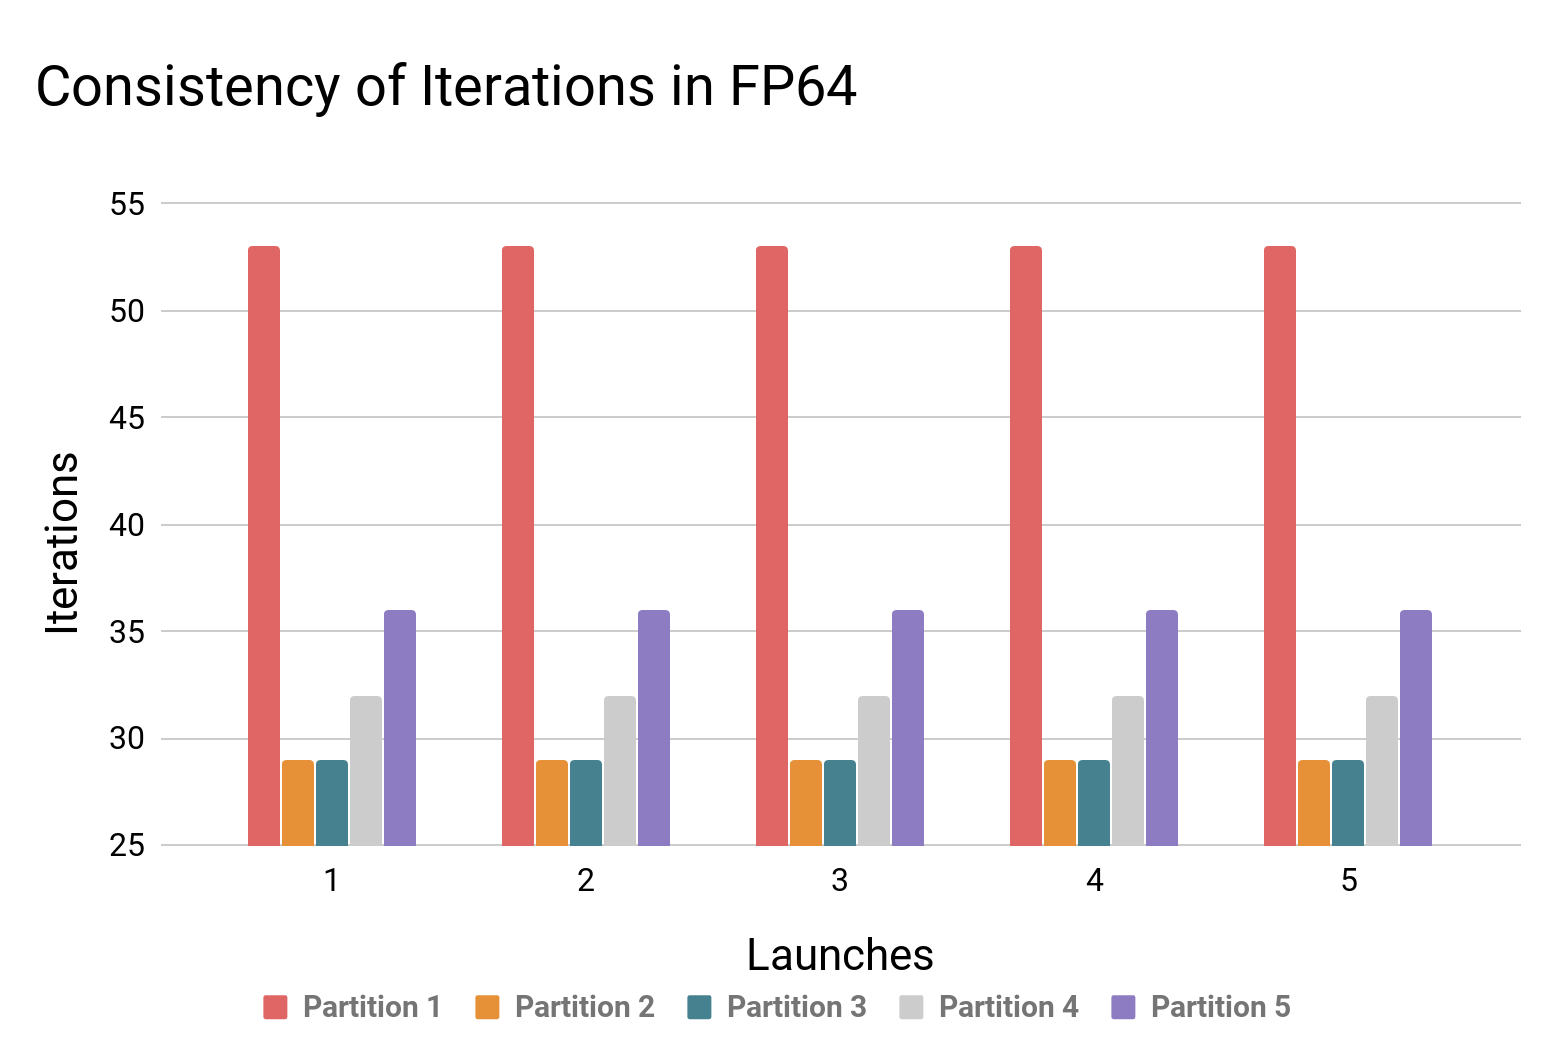
\includegraphics[width=.9\linewidth]{fp64consistency}
		\caption{Constant WLS iterations per partition}
		\label{fig:fp64consistency}
	\end{subfigure}
	\caption{WLS loop inconsistencies}
	\label{fig:mapooldmm}
\end{figure}

\subsection{Efficiency Evaluation}
The figures~\ref{fig:dsespeedupv100} and \ref{fig:dsespeedupgtx1070} show the speedups obtained using decentralized SE. The efficiency is found to increase with increase in size of the the grid as larger grids can be split into greater number of lighter subproblems that can be computed concurrently. 
\begin{figure}[H]
	\centering
	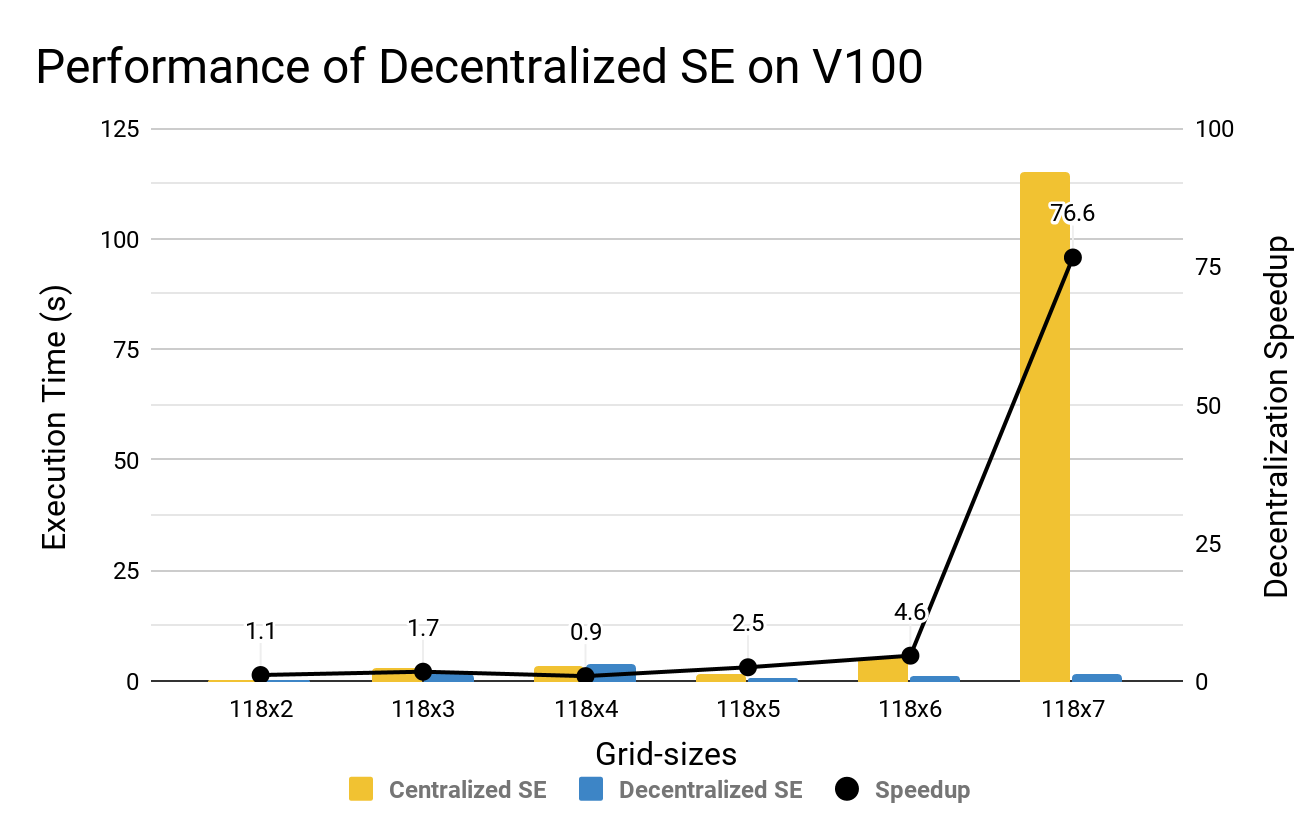
\includegraphics[scale=0.47]{dsespeedupv100}
	\caption{Speedup with decentralized SE against centralized SE on V100 GPU}
	\label{fig:dsespeedupv100}
\end{figure}

\begin{figure}[H]
	\centering
	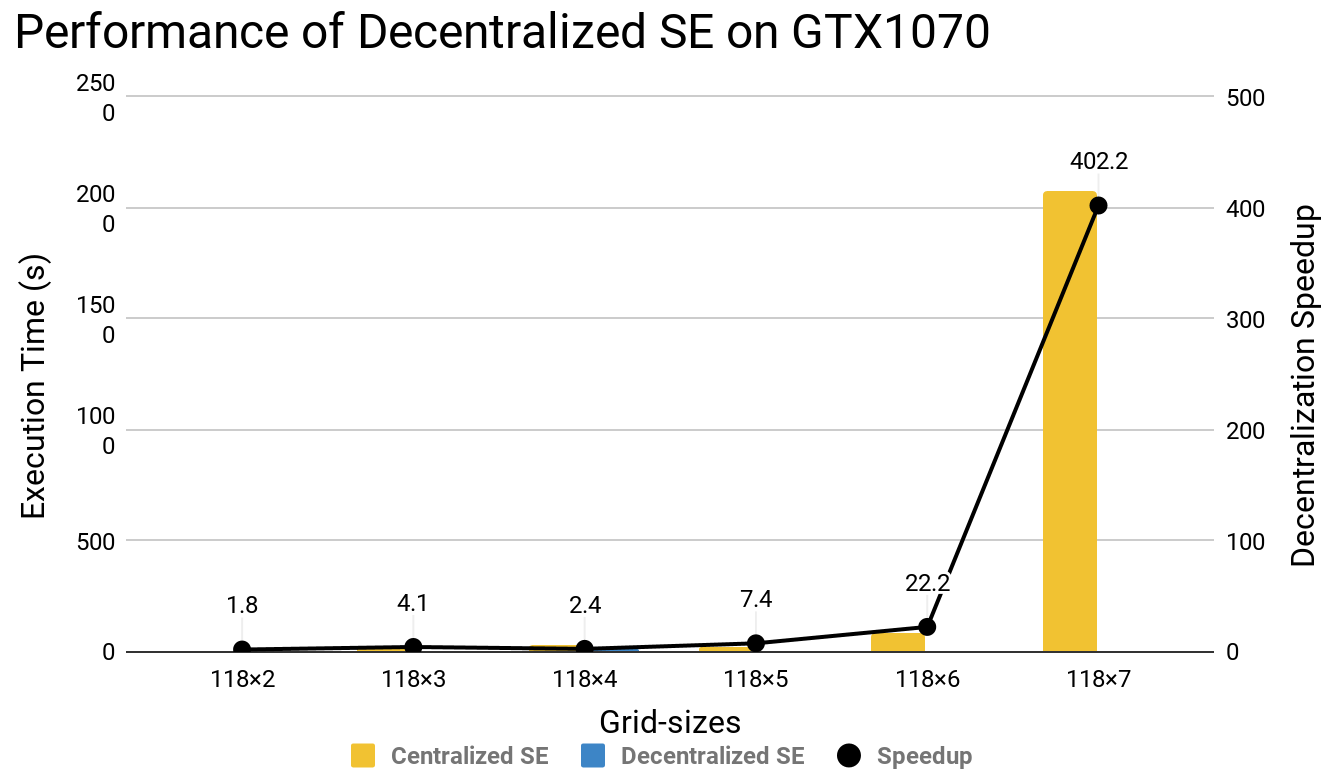
\includegraphics[scale=0.56]{dsespeedupgtx1070}
	\caption{Speedup with decentralized SE against centralized SE on GTX1070 GPU}
	\label{fig:dsespeedupgtx1070}
\end{figure}

\subsection{Reduction in Memory Requirements}
The memory requirements The table in Figure~\ref{fig:dsedevmemreduc} also shows the significant reduction in memory requirements for SE with decentralized approach. The memory consumption in case of centralized SE increases non-linearly whereas it remains almost linear for decentralized SE.
\begin{figure}[H]
	\centering
	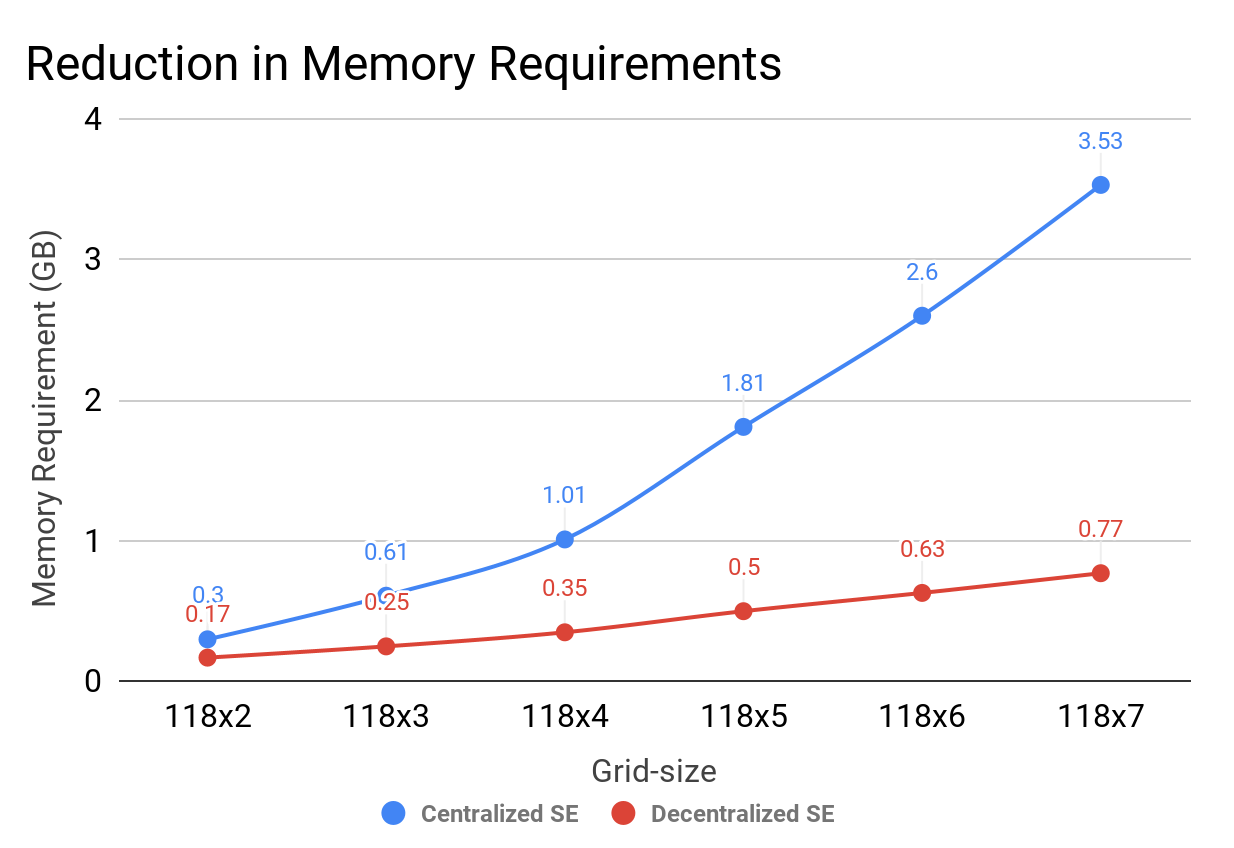
\includegraphics[scale=0.5]{dsedevmemreduc}
	\caption{Reduction in memory requirements due to decentralization of SE}
	\label{fig:dsedevmemreduc}
\end{figure}


\section{Evaluation Summary}
In this section, the overall inference of the results is provided. Based on the results, it is empirically evident that CUDA-accelerated decentralized SE delivers superior performance in comparison to CUDA-accelerated centralized SE. In practice, decentralization results in lower computational burden with higher speedups and lower memory requirements. Since only those grid-datasets with low merge-errors are considered for evaluation of decentralization, here the analysis of accuracy is not considered. The advantages of decentralization become crucial as the grid-size increases. The results from the analyses of centralized and decentralized SE are summarized in the tables~\ref{table:centralizedSEsummary} and \ref{table:decentralizedSEsummary} which are as follows:

{\renewcommand{\arraystretch}{1.3}%
\begin{table}[H]
	\centering
	\begin{tabular}{|r|r|r|r|r|r|r|}
		\hline
		\multicolumn{1}{|c|}{}                                                                                & \multicolumn{2}{c|}{\textbf{FP32 SE Speedup}}                              & \multicolumn{2}{c|}{\textbf{FP64 SE Speedup}}                              & \multicolumn{2}{c|}{\textbf{Required VRAM (GB)}}                              \\ \cline{2-7} 
		\multicolumn{1}{|c|}{\multirow{-2}{*}{\textbf{\begin{tabular}[c]{@{}c@{}}Grid \\ Size\end{tabular}}}} & \multicolumn{1}{c|}{\textbf{GTX1070}} & \multicolumn{1}{c|}{\textbf{V100}} & \multicolumn{1}{c|}{\textbf{GTX1070}} & \multicolumn{1}{c|}{\textbf{V100}} & \multicolumn{1}{c|}{\textbf{FP32 SE}} & \multicolumn{1}{c|}{\textbf{FP64 SE}} \\ \hline
		4                                                                                                     & {\color[HTML]{CB0000} 0.56}           & {\color[HTML]{009901} 1.20}        & {\color[HTML]{CB0000} 0.54}           & {\color[HTML]{009901} 1.12}        & 0.000023                              & 0.000046                              \\ \hline
		30                                                                                                    & {\color[HTML]{009901} 1.68}           & {\color[HTML]{009901} 2.46}        & {\color[HTML]{009901} 1.23}           & {\color[HTML]{009901} 2.67}        & 0.0018                                & 0.0035                                \\ \hline
		118                                                                                                   & {\color[HTML]{009901} 4.20}           & {\color[HTML]{009901} 5.12}        & {\color[HTML]{009901} 1.84}           & {\color[HTML]{009901} 5.18}        & 0.032                                 & 0.064                                 \\ \hline
		236                                                                                                   & {\color[HTML]{009901} 9.66}           & {\color[HTML]{009901} 12.60}       & {\color[HTML]{009901} 2.42}           & {\color[HTML]{009901} 12.08}       & 0.141                                 & 0.283                                 \\ \hline
		300                                                                                                   & {\color[HTML]{009901} 12.26}          & {\color[HTML]{009901} 15.42}       & {\color[HTML]{009901} 2.60}           & {\color[HTML]{009901} 13.28}       & 0.18                                  & 0.35                                  \\ \hline
		354                                                                                                   & {\color[HTML]{009901} 10.38}          & {\color[HTML]{009901} 14.30}       & {\color[HTML]{009901} 1.54}           & {\color[HTML]{009901} 13.17}       & 0.30                                  & 0.59                                  \\ \hline
		472                                                                                                   & {\color[HTML]{009901} 17.10}          & {\color[HTML]{009901} 26.65}       & {\color[HTML]{009901} 2.09}           & {\color[HTML]{009901} 21.24}       & 0.51                                  & 1.02                                  \\ \hline
		590                                                                                                   & {\color[HTML]{009901} 13.30}          & {\color[HTML]{009901} 28.27}       & {\color[HTML]{009901} 1.53}           & {\color[HTML]{009901} 20.73}       & 0.89                                  & 1.78                                  \\ \hline
		900                                                                                                   & {\color[HTML]{009901} 13.50}          & {\color[HTML]{009901} 35.44}       & {\color[HTML]{009901} 1.25}           & {\color[HTML]{009901} 22.68}       & 1.73                                  & 3.46                                  \\ \hline
		1500                                                                                                  & {\color[HTML]{009901} 13.12}          & {\color[HTML]{009901} 30.92}       & {\color[HTML]{CB0000} \textbf{-1}}    & {\color[HTML]{009901} 19.90}       & 4.81                                  & 9.62                                  \\ \hline
	\end{tabular}
	\caption{Speedups and memory consumption through centralized SE against serial algorithm}
	\subcaption*{Speedups larger than 1 are desirable. -1 indicates program crash due to insufficient VRAM.}
	\label{table:centralizedSEsummary}
\end{table}}


{\renewcommand{\arraystretch}{1.3}%
% Please add the following required packages to your document preamble:
% \usepackage{multirow}
% \usepackage[table,xcdraw]{xcolor}
% If you use beamer only pass "xcolor=table" option, i.e. \documentclass[xcolor=table]{beamer}
\begin{table}[H]
	\centering
	\begin{tabular}{|l|r|r|r|r|r|r|r|r|}
		\hline
		\multicolumn{1}{|c|}{}                                                                               & \multicolumn{3}{c|}{\textbf{V100}}                                                                                              & \multicolumn{3}{c|}{\textbf{GTX1070}}                                                                                           & \multicolumn{2}{c|}{\textbf{\begin{tabular}[c]{@{}c@{}}VRAM\\ (GB)\end{tabular}}}                \\ \cline{2-9} 
		\multicolumn{1}{|c|}{}                                                                               & \multicolumn{2}{c|}{\textbf{Time (s)}}                                & \multicolumn{1}{l|}{}                                   & \multicolumn{2}{c|}{\textbf{Time (s)}}                                & \multicolumn{1}{l|}{}                                   & \multicolumn{1}{c|}{}                               & \multicolumn{1}{c|}{}                               \\ \cline{2-3} \cline{5-6}
		\multicolumn{1}{|c|}{\multirow{-3}{*}{\textbf{\begin{tabular}[c]{@{}c@{}}Grid\\ Size\end{tabular}}}} & \multicolumn{1}{c|}{\textbf{cSE}} & \multicolumn{1}{c|}{\textbf{dSE}} & \multicolumn{1}{l|}{\multirow{-2}{*}{\textbf{Speedup}}} & \multicolumn{1}{c|}{\textbf{cSE}} & \multicolumn{1}{c|}{\textbf{dSE}} & \multicolumn{1}{l|}{\multirow{-2}{*}{\textbf{Speedup}}} & \multicolumn{1}{c|}{\multirow{-2}{*}{\textbf{cSE}}} & \multicolumn{1}{c|}{\multirow{-2}{*}{\textbf{dSE}}} \\ \hline
		118$\times$2                                                                                                & 0.26                              & 0.23                              & {\color[HTML]{009901} 1.1}                              & 1.1                               & 0.6                               & {\color[HTML]{009901} 1.8}                              & 0.3                                                 & 0.17                                                \\ \hline
		118$\times$3                                                                                                & 2.77                              & 1.60                              & {\color[HTML]{009901} 1.7}                              & 19.7                              & 4.8                               & {\color[HTML]{009901} 4.1}                              & 0.61                                                & 0.25                                                \\ \hline
		118$\times$4                                                                                                & 3.3                               & 3.7                               & {\color[HTML]{CB0000} 0.9}                              & 32.7                              & 13.6                              & {\color[HTML]{009901} 2.4}                              & 1.01                                                & 0.35                                                \\ \hline
		118$\times$5                                                                                                & 1.5                               & 0.61                              & {\color[HTML]{009901} 2.5}                              & 20                                & 2.7                               & {\color[HTML]{009901} 7.4}                              & 1.81                                                & 0.5                                                 \\ \hline
		118$\times$6                                                                                                & 5.1                               & 1.1                               & {\color[HTML]{009901} 4.6}                              & 86.7                              & 3.9                               & {\color[HTML]{009901} 22.2}                             & 2.6                                                 & 0.63                                                \\ \hline
		118$\times$7                                                                                                & 114.9                             & 1.5                               & {\color[HTML]{009901} 76.6}                             &    2079.1                               &   5.17                                &  {\color[HTML]{009901} 402.2}                                                         & 3.53                                                & 0.77                                                \\ \hline
	\end{tabular}
	\caption{Speedups through decentralized FP64 SE (dSE) against centralized FP64 SE (cSE)}
	\subcaption*{Speedups larger than 1 are desirable. Decentralized SE is predominantly quicker due to reduced order of matrices.}
	\label{table:decentralizedSEsummary}
\end{table}}

\subfilebib % Makes bibliography available when compiling as subfile
\end{document}